\documentclass[letterpaper,11pt]{article}

\usepackage{geometry}
\usepackage{pslatex}
\usepackage{fancyhdr}
\usepackage{graphicx}
\usepackage{color}
\usepackage{enumitem} % for ordered list labels
\usepackage{amssymb} % for symbols
\usepackage{scrextend} % for indentation
\usepackage{tabto} % for tabs
\usepackage{amsmath} % for text in equation
\usepackage{listings} % to highlight code
\usepackage{forest, tikz} % to make forest

% Define a custom color
\definecolor{backcolour}{rgb}{0.95,0.95,0.92}
\definecolor{codegreen}{rgb}{0,0.6,0}

% Define a custom style
\lstdefinestyle{myStyle}{
    backgroundcolor=\color{backcolour},   
    commentstyle=\color{codegreen},
    basicstyle=\ttfamily\footnotesize,
    breakatwhitespace=false,         
    breaklines=true,                 
    keepspaces=true,                 
    numbers=left,       
    numbersep=5pt,                  
    showspaces=false,                
    showstringspaces=false,
    showtabs=false,                  
    tabsize=2,
}

% Use \lstset to make myStyle the global default
\lstset{style=myStyle}

\graphicspath{ {./} }
\geometry{ margin = 1.0in }

%%% TODO modify these variables %%%
\def\homeworknum{5}
\def\myname{Harshit Jain}
\def\myaccessid{hmj5262}
\def\myrecitation{8}
%%%%

\pagestyle{fancy}
\lhead{{\bf CMPSC 465 Fall 2022}}
\chead{{\bf Assignment~\homeworknum}}
\rhead{{\bf \today}}

\newcounter{problemid}
%\stepcounter{problemid}
\def\newproblem{\clearpage\newpage{\bf Problem~\arabic{problemid}\stepcounter{problemid}}\hfill\fbox{\parbox{0.16\textwidth}{\bf Points:}}\par}

\setlength\parindent{0em}
\setlength\parskip{8pt}
\setlength{\fboxsep}{6pt}


\begin{document}

\framebox[\textwidth]{
	\parbox{0.96\textwidth}{
		\parbox{0.12\textwidth}{\bf Name:}\parbox{0.6\textwidth}{\myname}\\
		\parbox{0.12\textwidth}{\bf Access ID:}\parbox{0.6\textwidth}{\myaccessid}\\
		\parbox{0.12\textwidth}{\bf Recitation:}\parbox{0.6\textwidth}{\myrecitation}
	}
}


%% your solutions %%%

\newproblem
\textbf{Acknowledgements}
\begin{enumerate}[label=(\alph*)]
    \item I did not work in a group.
    \item I did not consult without anyone my group members.
    \item I did not consult any non-class materials.
\end{enumerate}


% PROBLEM 1
\newproblem
\textbf{DFS Basics}
\begin{enumerate}[label=(\alph*)]
    
    \item $A \rightarrow B \rightarrow D \rightarrow E \rightarrow G \rightarrow F \rightarrow C \rightarrow H \rightarrow I$ 
    
    \item 
    \begin{minipage}{.22 \linewidth}

		\begin{tabular}{l | l}
        
		$A$ & $(1,12)$\\
		$B$ & $(2,11)$\\
		$C$ & $(13,18)$\\
		$D$ & $(3,6)$\\
		$E$ & $(4,5)$\\
		$F$ & $(8,9)$\\
		$G$ & $(7,10)$\\
		$H$ & $(14,17)$\\
		$I$ & $(15,16)$ \\
		\end{tabular}\\ 
	\end{minipage}

    \item 
    \begin{minipage}{.22 \linewidth}

		\begin{tabular}{l | l}
        
		\textbf{Edge} & \textbf{Type}\\
		$(A,B)$ & Tree\\
		$(A,E)$ & Forward\\
		$(B,D)$ & Tree\\
		$(D,E)$ & Tree\\
		$(E,D)$ & Back\\
		$(B,G)$ & Tree\\
		$(G,F)$ & Tree\\
		$(G,D)$ & Cross\\
		$(C,H)$ & Tree\\
		$(H,I)$ & Tree\\
		$(C,I)$ & Forward\\
		\end{tabular}\\ 
	\end{minipage}

\end{enumerate}



% PROBLEM 2
\newproblem
\textbf{Pre and Post Processing}
\begin{enumerate}[label=(\alph*)]
    
    \item 
    For our DFS algorithm, if post$(u) <$ post$(v)$, then, 

    \begin{itemize}

        \item Case $1: [\text{pre}(u), \text{post}(u)] [\text{pre}(v), \text{post}(v)]$

        \item Case $2: [\text{pre}(v), [\text{pre}(u), \text{post}(u)] \text{post}(v)]$

    \end{itemize}
    
    These are the only $2$ Cases for an undirected graph where post$(u) <$ post$(v)$.

    Since we know there is an edge between these $2$ nodes, Case $1$ can not happen because we must visit all the neighbors
    of a node before marking it as visited. That means, in Case $1$, node $u$ is marked visited before exploring edge $v$ as
    it has post$(u) <$ post$(v)$ which is violating the DFS rule of exploring all neighbor nodes before marking it visited.
    So, Case $2$ is the only possible one, which yields $v$ as the ancestor of $u$. The statement is True.

    \item 

    First, Run Depth First Search Algorithm on the tree while also keeping the timestamps for the time when $u$ is started to
    get explored (pre-number) and the time when $u$ is finished getting explored (post-number). For every node $u$, pre$(u)$
    denotes the time when we began exploring $u$ and post$(u)$ denote the time when we finished it. This process will take linear
    time since the $Explore()$ function will never be called on a Node more than once.

    Now, to check whether $u$ an ancestor of $v$, we have to check whether:

    \[\text{pre}(u)<\text{pre}(v) \text{ and post}(u)>\text{post}(v)\]

    If the above condition becomes True, then $u$ is the ancestor of $v$. This condition will itself take a constant time becuase
    it is just comparing two numbers.

    

\end{enumerate}


% PROBLEM 3
\newproblem
\textbf{Linearization Basics}
\begin{enumerate}[label=(\alph*)]
    
    \item 
    \begin{minipage}{.22 \linewidth}

		\begin{tabular}{l | l}
        
		$A$ & $(1,14)$\\
		$B$ & $(15,16)$\\
		$C$ & $(2,13)$\\
		$D$ & $(3,10)$\\
		$E$ & $(11,12)$\\
		$F$ & $(4,9)$\\
		$G$ & $(5,6)$\\
		$H$ & $(7,8)$\\
		\end{tabular}\\ 
	\end{minipage}

    \item
    Sources $:A,B$ $(A,B$ are having most elevated post number$)$

    Sinks $:G,H$ $(G,H$ are having least post number$)$

    \item 
    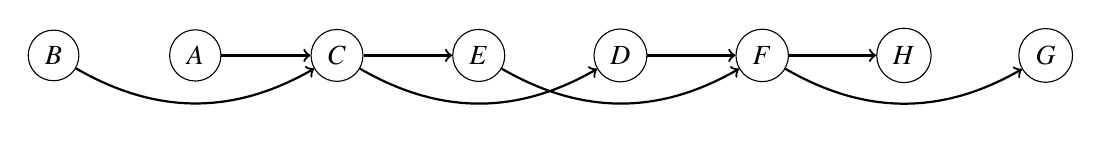
\begin{tikzpicture}[scale=0.9,auto=center]
        \node[circle, draw] (b) at (0, 0) {$B$};
        \node[circle, draw] (a) at (2, 0) {$A$};
        \node[circle, draw] (c) at (4, 0) {$C$};
        \node[circle, draw] (e) at (6, 0) {$E$};
        \node[circle, draw] (d) at (8, 0) {$D$};
        \node[circle, draw] (f) at (10, 0) {$F$};
        \node[circle, draw] (h) at (12, 0) {$H$};
        \node[circle, draw] (g) at (14, 0) {$G$};

        \draw[->, thick] (b) to[bend right] (c);
        \draw[->, thick] (a) to (c);
        \draw[->, thick] (c) to (e);
        \draw[->, thick] (c) to[bend right] (d);
        \draw[->, thick] (d) to (f);
        \draw[->, thick] (e) to[bend right] (f);
        \draw[->, thick] (f) to (h);
        \draw[->, thick] (f) to[bend right] (g);
        
    \end{tikzpicture}

    \item 
    We have three times where we can choose between two vertices on a path so $2^{3} = 8$ lenearization.
\end{enumerate}
\end{document} 
